\chapter{FEA data management}
\label{chapter:data-management}

Together with growing complexity of finite element calculations, the importance of management of data produced by the calculations is increasingly emphasized in both industrial and research communities. Information is often shared between multiple users, moved from one computer to another, and further transformed to enable different views over the data. Some definition of persistent and standard representation of the data is therefore required as well as the corresponding data access system architecture that allows to query the data.

\section{System architecture}
\label{sec:system-architecture}

The prototype implementation of the FEA data management system is designed as a collaborative framework that can be accessed by users from different client devices. Figure \ref{fig:FEA-architecture} depicts the schema of the system architecture. System consists of several independent modules. The FEM calculation itself runs on a remote server as one of micro-services\footnote{\todo{TODO: micro-services}} along with mesh generation service, results processing service, etc. These services are controlled by the application service that provides interface to the client applications in form of REST-ful web API\footnote{\todo{TODO: REST; REST-ful service; REST web API.}}.

\begin{figure}[H]
    \centering
    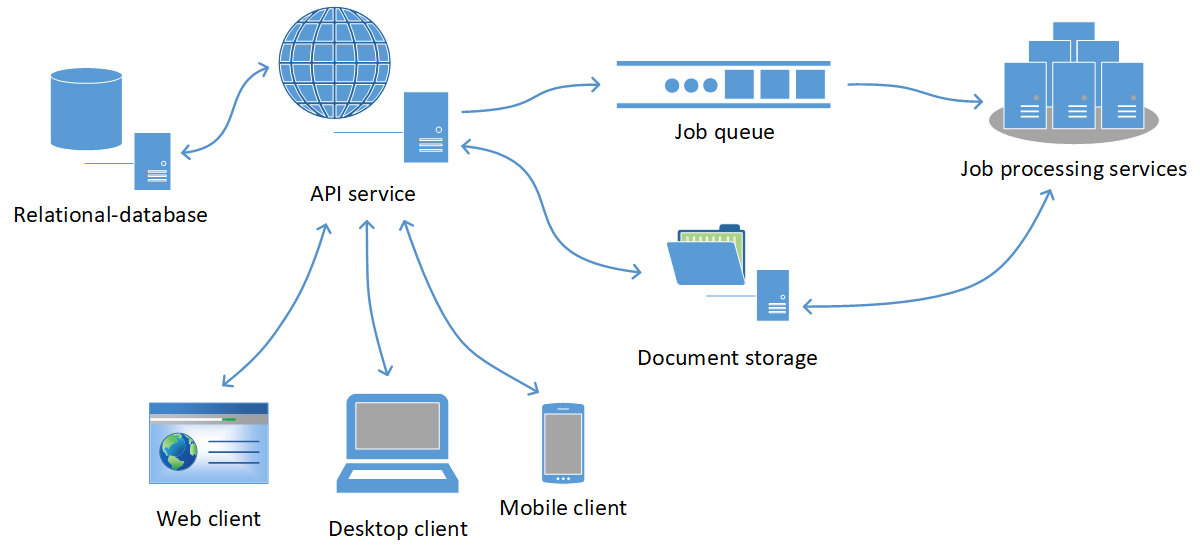
\includegraphics[width=\textwidth]{figures/chapter-data-management/FEA-architecture}
    \decoRule
    \caption{FEA system architecture.}
    \label{fig:FEA-architecture}
\end{figure}

The architecture relies on an abstraction provided by Platform-as-a-Service\footnote{\todo{PaaS. TODO: These services can be carried in a public cloud or on-premises. https://azure.microsoft.com/en-us/overview/what-is-paas/ ...}} computing model. No service component is tied directly to a specific machine. Hardware resources are allocated when they are needed by a service infrastructure controller. This makes the scaling and deployment of components easier and allows to focus on the problem domain instead of solving server configuration and networking issues.

The system contains two types of data storage. The relational-database type of storage is intended to store basic project-related data such as description of simulations, links to the simulation resources, information about the owner and other colaborating users, etc. The input to the FEA -- geometrical model, attribute assignments, and analysis parameters -- can also be stored in a relational database, eventhough, storing this complex type of information in the SQL database is questionable and has its drawbacks\footnote{\todo{TODO: Zminit vyhody i nevyhody. Jake jsou alternativy? No-SQL databaze?}}.

The second type of storage is a blob storage\footnote{Blob storage is also referred to as Object storage. It is a service for storing large amounts of unstructured object data, that can be accessed over the network via HTTP or HTTPS. A blob can be any type of text or binary data, such as document or media files. Blob is an acronym for Binary Large OBject.} used to hold temporary files serving as the input or the output to particular components, especially the mesh generator and the FEM solver. The system is designed to be independent of the solver and mesh generator components, therefore this intermediate step of converting the input to proprietary file format that the components understand is necessary. In the future, it is possible to expect a gradual transition from the file-based approach to the direct connection to the database and query the input model directly. Also, the output of the calculation could be saved directly in the proposed format to represent the results in post-process-ready form.

Workflow diagram in Figure \ref{fig:FEA-workflow} helps to visualize the sequence of FEA steps and the transfer of data between the service components. It also reveals the basic design principle behind the microservice architecture -- Separation of concerns\footnote{Separation of concerns -- design principle for separating system into distinct sections, such that each section addresses a separate concern.}. The vertical bars denote computational intensive tasks performed by the service components. The client side in the diagram represents the presentation layer of the FEA system that the user directly interacts with. In the presentation layer, also called \textit{frontend}, there is spent the vast majority of time by users doing pre- and post-processing of data (which is not depicted in the diagram). The Web API service, also called as \textit{backend}, is the key component that assigns work to other components, serves as an controller for a running analysis and mainly as an interface between the data stored in databases and the client applications.

\begin{figure}[H]
    \centering
    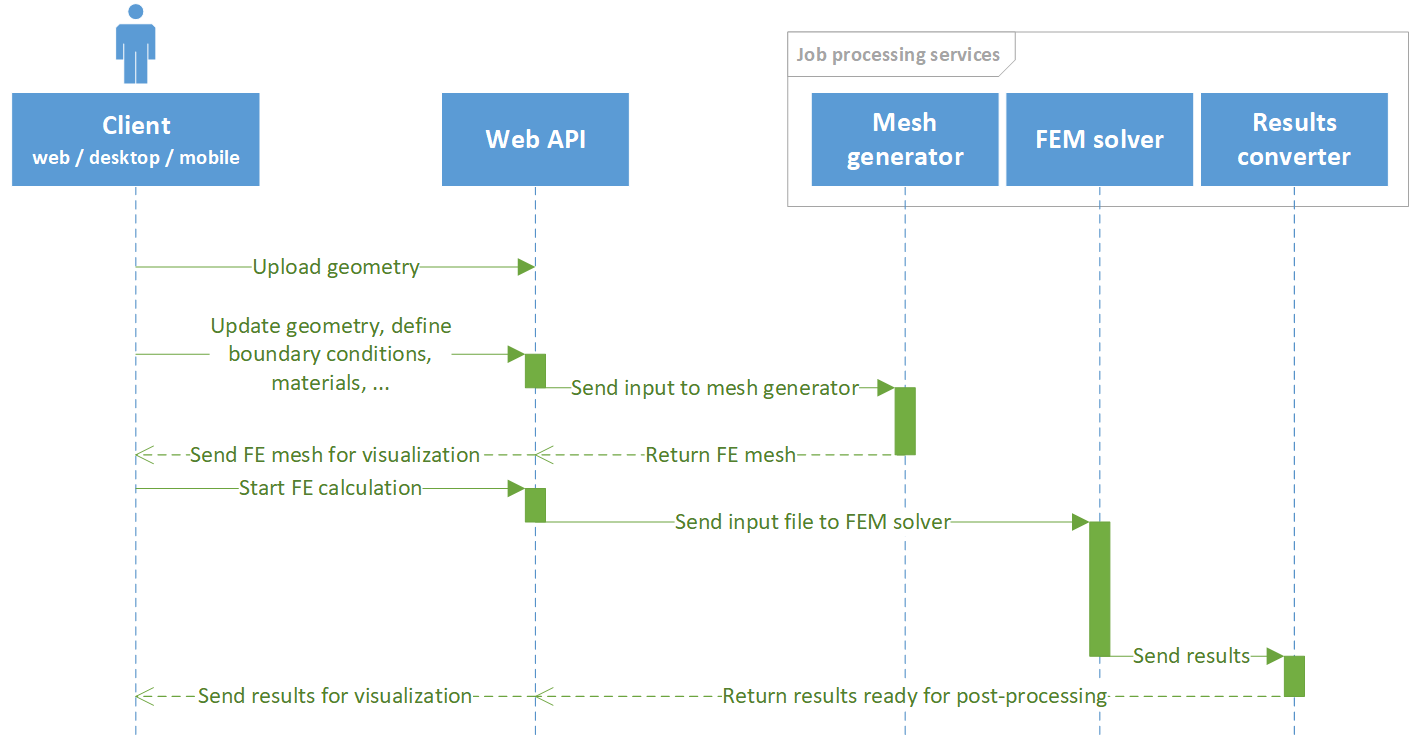
\includegraphics[width=\textwidth]{figures/chapter-data-management/FEA-workflow}
    \decoRule
    \caption{FEA system workflow.}
    \label{fig:FEA-workflow}
\end{figure}

The prototype implementation of the data management system follows the schema and the workflow depicted in Figures \ref{fig:FEA-architecture} and \ref{fig:FEA-workflow}. The difference is that the pre-processing phase is currently excluded. The focus of the work presented in this thesis is primarily on the post-processing features and the representation of results. Therefore, the results from the existing FEM solver are uploaded into the system and the system converts them to the internal representation suitable for post-processing. To test the prototype implementation of the data management system, two client applications are created. The first is the feature-rich desktop post-processor with the support for Microsoft Windows and Linux operating systems. The second is the simple web application that provides basic control over an analysis and basic post-processing capabilities. Its purpose is mainly to demonstrate the benefits of proposed format for storage of results when post-processing complex FEA. Its web-based implementation allows for truly cross-platform experience without the need for installation and it allows to access the analysis data even from low-end mobile devices.

\section{Project-based data representation}
\label{sec:project-db-schema}

Most researchers and engineers typically work independently using their own workstations, while sharing the hardware infrastructure for intensive FEM calculations. The output from the complex analyses are also shared as it would be costly and ineffective if each collaborator had performed her/his own calculations. Since potentially many users can access the server to oversee the analysis and to query the analysis results, a project management scheme is needed. The overall database schema is depicted in Figure \ref{fig:FEA-db-schema}. It is an entity-relationship diagram representing conceptual model that can be mapped on the SQL database model.

\begin{figure}[H]
    \centering
    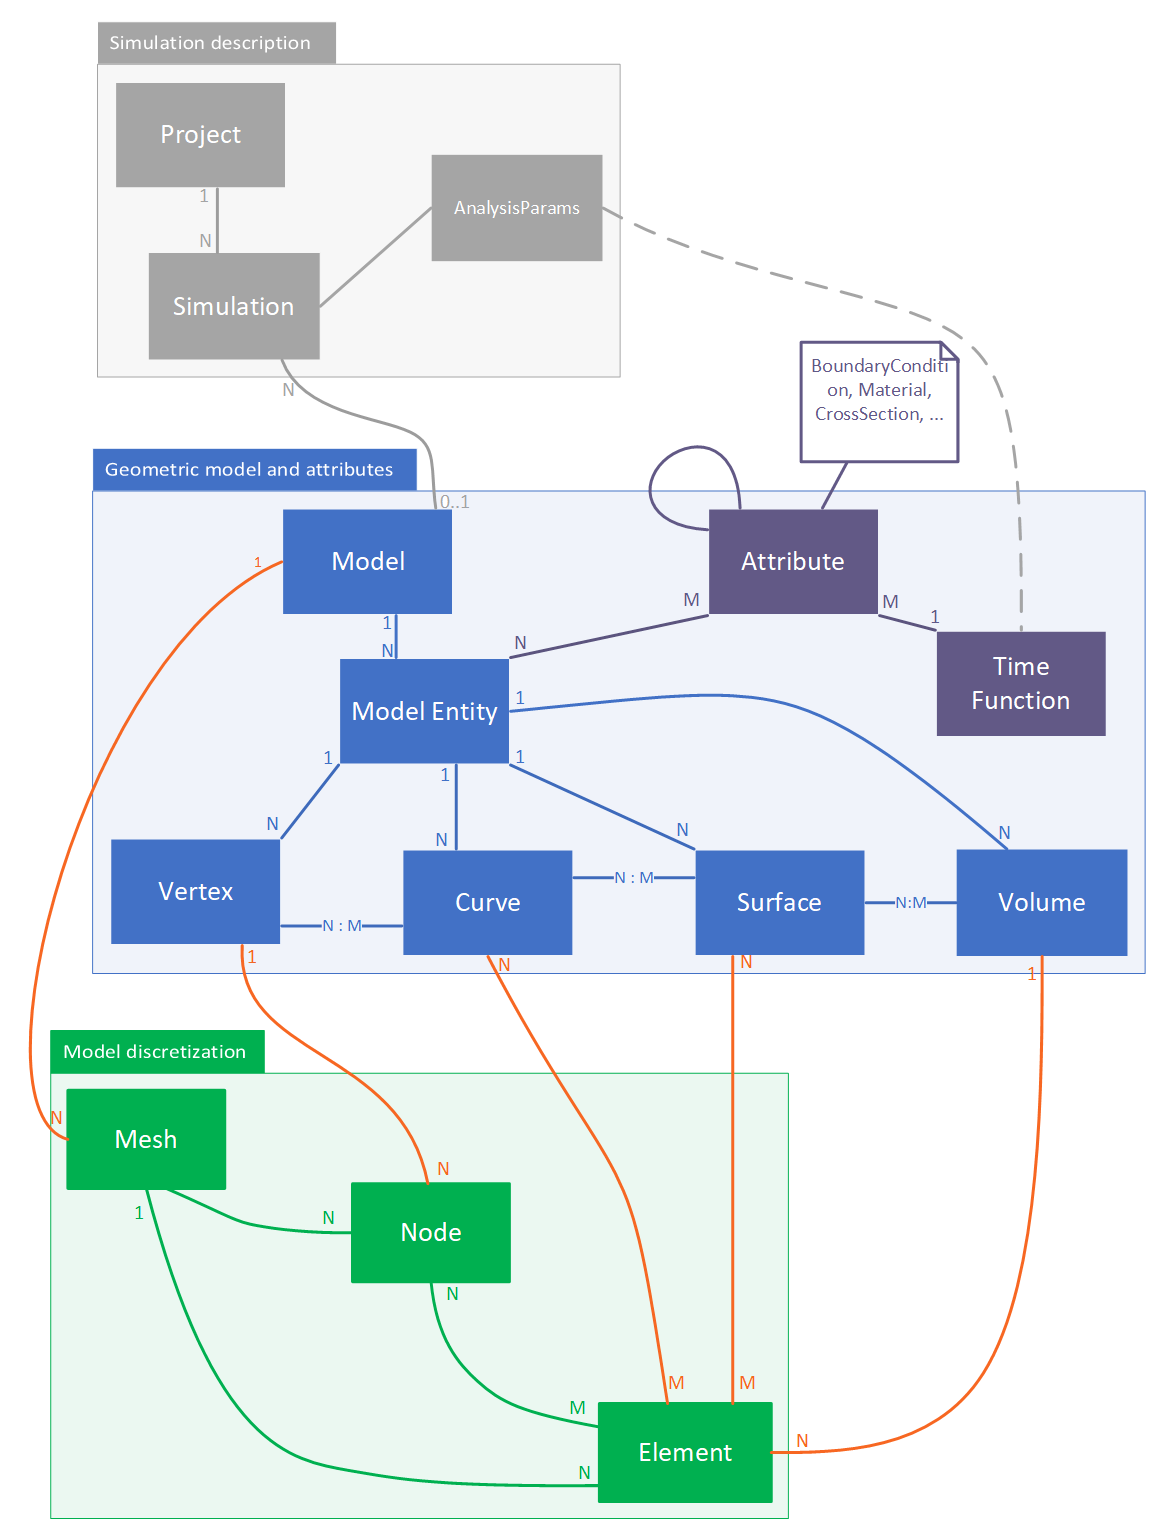
\includegraphics[width=0.8\textwidth]{figures/chapter-data-management/FEA-database-schema}
    \decoRule
    \caption{Database schema for FEA.}
    \label{fig:FEA-db-schema}
\end{figure}

The Project entity holds the basic information about a set of related analyses. It has name, the owner, and the list of other users that have access permissions. The Project has also relations to the list of simulations. The Simulation entity encapsulates the information about a single finite element analysis. Each simulation can have different input -- geometrical model, attributes (properties of model entities, i.e., material properties of volumes, initial and boundary conditions), and/or parameters of analysis (e.g., number of time steps). Geometrical model and its discretizations (finite element meshes) can either be stored directly in a relational database or as a custom file in a blob storage.

% Doplnit tuto kapitolu nejakym textem o projektovych datech / o vstupnim modelu, OOFEM-link, db ...

\section{Storage format for results}
\label{sec:storage-format}

% Pojmout tuto kapitolu jako detailni specifikaci formatu. Inspirovat se dokumentem GiD postprocess format (a take mozna C# proposals na githubu)

The conceptual model presented in Figure \ref{fig:FEA-db-schema} can be naturally extended with the entities representing the results of the simulations. The project-based data model enhanced with the representation of simulation results is depicted in Figure \ref{fig:FEA-db-schema-results} as ER diagram. The corresponding class diagram is depicted in Figure \ref{fig:results-class-diagram}, which describes the object representation of the Solution entity. It is physically representated either by a JSON file in local file system or by several tables in relational database.

\begin{figure}[H]
    \centering
    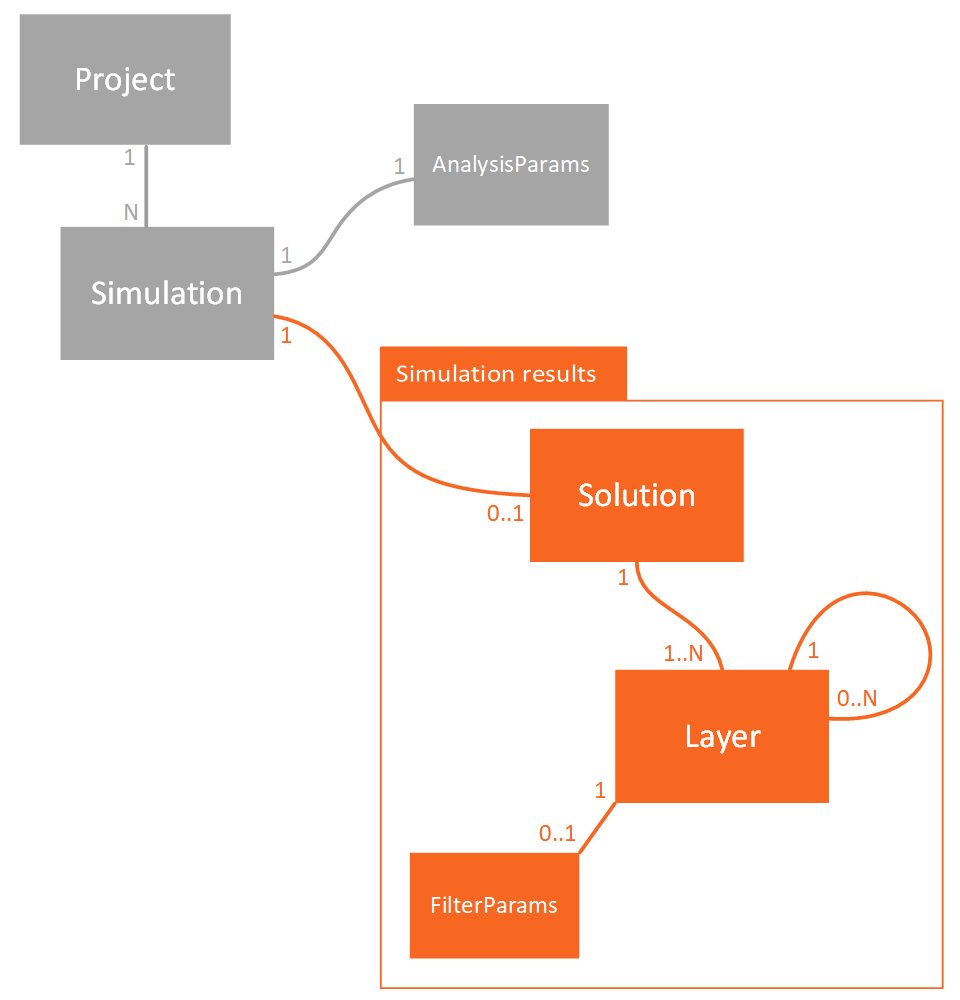
\includegraphics[width=0.8\textwidth]{figures/chapter-data-management/FEA-database-schema-only-results}
    \decoRule
    \caption[Database schema for FEA with results representation only]{Database schema for FEA with results representation only (without the input model).}
    \label{fig:FEA-db-schema-results}
\end{figure}

\begin{figure}[H]
    \centering
    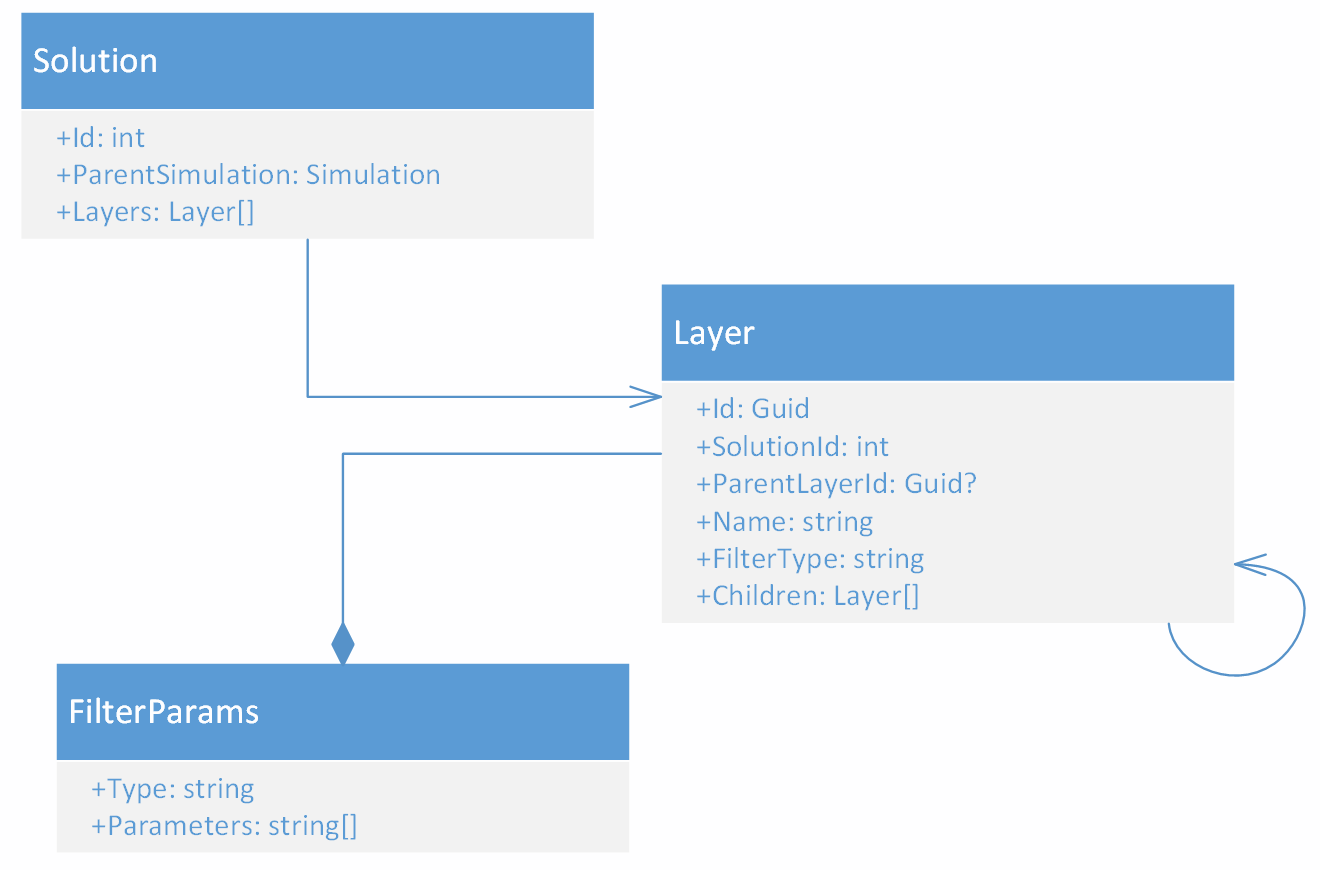
\includegraphics[width=0.8\textwidth]{figures/chapter-data-management/results-class-diagram}
    \decoRule
    \caption{Object representation of simulation results.}
    \label{fig:results-class-diagram}
\end{figure}

The simulation results are represented by the Solution entity, which holds a structure representing the results from a FEM solver that are converted to the form suitable for post-processing. The structure has the form of a tree. A node of the tree is represented by the Layer entity. A layer is an association of a mesh and corresponding result fields and other attributes. The use of tree structure allows to preserve the relations between the parent layers and the layers that were derived from them. The mesh that is referenced by a layer need not be the same as the mesh used as the input mesh to the FEM solver. It could be modified by the solver during the calculation, e.g. due to the use of adaptive finite element techniques \footnote{\todo{TODO: ... which can automatically refine, coarsen, or relocate a mesh to achieve a solution having a specified accuracy}}. Also, the resulting mesh can be further modified to facilitate the post-processor implementation, e.g. the surface representation of a 3D mesh can be generated. Also a number of cross-sections can created at uniform intervals to provide a look inside the mesh. Generally, multiple views on the results can be prepared in advance before the user even starts to investigate the results.

The concept of a layer is not new. It is used in existing implementations of the post-processors in FEA software packages (often named \textit{filter} instead of layer), to represent a view on the results. However, the layers (visual filters) are usually generated on demand by specific user request and they are not kept in a persistent storage. The proposed storage format for results is built on top of layer tree structure directly, which allows layers to be accessed later on, even on a different device, or shared by multiple users working on the same project.

In the prototype implementation of the FEA data management system, it is supposed that the FEM solver uses its own proprietary format to represent the result from the simulation. As the system is designed to be independent of individual components, the Results converter component converts the results from the FEA solver into the standardized layer-based format suitable for post-processing. The specification of the format follows.

\subsection{Format specification}

All documents that participate in the storage format are presented in JSON format. JSON is the today's standard for data transport in web technologies and also as a storage format in currently popular NoSQL\footnote{\todo{TODO: NoSQL ... Stands for Not-only SQL ...}} databases. It is a consise textual format easily readable both for a human and for a computer. However, the storage format is not tightly coupled with JSON, data can be encoded in another structured format, such as XML. Also, as mentioned above in the text, there are two types of locations the data can be stored in -- \textbf{remote} and \textbf{local}. Both locations are supported in the prototype implementation. In either case the key part of the format is a solution document. An example of the solution document is given in Listing \ref{lst:solution.json}. In case of the remote storage, the solution document is stored in a relational database as part of the project-based data representation shown in Figure \ref{fig:FEA-db-schema-results}, while the rest of documents are stored in a blob storage as group of JSON documents. In case of the local storage, all documents, including the solution, are stored in a folder as JSON files in local file system on a personal computer on which the results are post-processed.

As can be seen in the example of the solution document in Listing \ref{lst:solution.json}, each layer is assigned a unique identifier, specifically a GUID\footnote{\todo{TODO: GUID... Globally unique identifier, sometimes the term UUID is used ... 128bit, 4bits reserved for version ...}} number. A GUID in its textual representation is also used to unambigously determine the location of the layer documents. In case of a solution stored locally, a GUID is used as a name of the folder the related layer documents are stored in. For remote solutions, a GUID is used as a part of a URL when requesting resources from a database or a blob storage.

% TODO: describe properties in solution document? Id, ProjectName, Location, Results, Layers, Layers.Id, Layers.Name, Layers.FilterType, Layers.Children

Data in each layer are stored in four types of documents. All documents are identified by a layer id and by its index within the layer (except Summary document that does not need an index as it exist in one copy per layer).
\begin{itemize}

    \item \textbf{Summary document} contains all the descriptive information about the layer. An example of a summary document in JSON format is presented in Listing \ref{lst:summary.json}. Besides a unique id, a layer has its name, which the user can choose arbitrarily, otherwise it is automatically derived from the \code{Filter} property. \code{Filter} property describes the parameters of the transformation applied to the parent layer to obtain the current layer. \code{ParentId} property contains the GUID assigned to the parent layer. The topmost root of the layer tree has no parent. Therefore, its \code{ParentId} property is null as well as \code{Filter} property. Default name for the root layer is ``master''\footnote{The format allows the existence of multiple \textit{master} layers, but it turns out that it is not necessary in practice. In the vast majority of cases, there is a single root layer and it is called ``master''.}.

    \code{Meshes} property holds a collection of mesh descriptors. A mesh descriptor serves as an reference to an actual mesh document related to a layer. Each mesh in a layer is assigned an index. It is a number that uniquely identifies the mesh within the layer. \code{TimeSteps} property of each mesh contains the list of time steps for which the mesh is defined. In usual case there is only one mesh for all time steps. In some cases, however, there can be different mesh for each time step. Application of deformation filter on a layer yields a derived layer that contains the same number of meshes as is the number of time steps, because the deformed meshes are generated by translating the nodes of the parent mesh by displacements calculated for each time step. Even the master layer can be composed of multiple meshes, e.g. when representing the results from a simulation of construction stages. The time step number must be a unique floating-point number as it serve as an identifier.
    
    Each mesh has optional set of attributes. An attribute is an umbrella term for additional information assigned to mesh entities. It is usually a property of the input model that is propagated to the results as it can be interesting during post-processing. The most common attribute is the material number that is assigned to each element of the mesh.

    \code{Fields} property contains a dictionary of result descriptors. Each field descriptor is introduced by the name of the field imported from the FEM results. Field can be composed of one or more components. Similarly, each component descriptor is identified by its name and enumerates the time steps in which the component is defined. Each time step descriptor contains the index of the corresponding result document as well as the index of the mesh document. Each result document always contains data for only one data component. However, the format allows that the data from multiple time steps can be gathered and stored in a single result document. The compression can be then applied on the range of time steps as a whole to achive better compression ratio. Therefore, to recover an arbitrary data component located either in a local or in a remote storage, the post-processor needs just a triplet of identifiers -- the layer id, the index of a result document, and the time step.

    \item \textbf{Mesh document} contains the geometric representation of a finite element mesh. An example of a mesh document in JSON format is presented in Listing \ref{lst:mesh.json}. Positions of the nodes are encoded in \code{PointCoordinates} property\footnote{Note that the terms \textit{node} and \textit{element} are internally referred to by more general terms \textit{point} and \textit{cell}.\label{foot:points-cells}}. Position of each node is a vector, whose components are floating-point numbers. Number of vector components is equal to the number of dimensions of the mesh. Vector components are flattened into a one dimensional array and converted to text using binary-to-text encoding (more about encoding in Section \ref{subsec:encoding}). \code{CellConnectivity} property\footnotemark[\getrefnumber{foot:points-cells}] contains encoded list of indices of element nodes that point to the coordinate array. The number of nodes per element can be retrieved by decoding \code{CellTypes} property, in which the types of all elements are stored. The supported element types along with their identifiers are depicted in Figure \ref{fig:supported-cell-types}. The identifiers are 8-bit unsigned integers (bytes) and the values match the definition of cell types in VTK file format \cite{XXX-vtk-file-format-pdf} to provide basic compatibility and to ease the conversion from the VTK format.
    
    \begin{figure}[H]
        \centering
        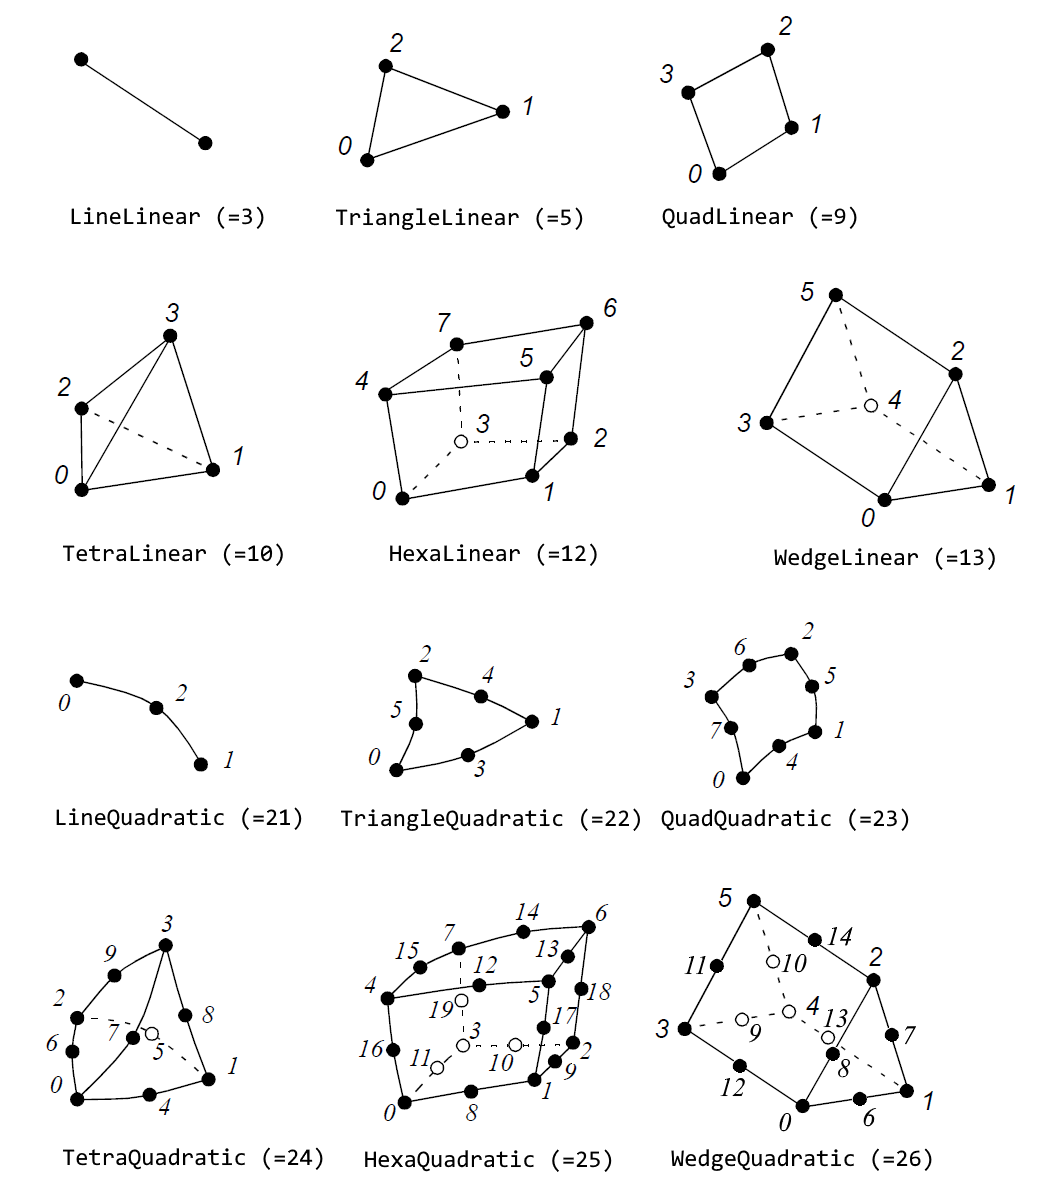
\includegraphics[width=0.9\textwidth]{figures/chapter-data-management/supported-cell-types}
        \decoRule
        \caption[Element types supported in storage format]{Element types supported in storage format. The values used for encoding element types in CellTypes array are shown in parentheses. The illustrations of elements are taken from \cite{XXX-vtk-file-format-pdf}.}
        \label{fig:supported-cell-types}
    \end{figure}
    
    Properties \code{Center} and \code{Radius}, eventhough their values can be calculated from the coordinate array, were added as an performance optimization for a post-processor since it is usually needed to normalize the mesh dimensions before the first rendering.

    \item \textbf{Attribute document} serves as a container for additional information assigned to mesh entities, e.g. material id of each finite element. An example of a attribute document in JSON format is presented in Listing \ref{lst:attribute.json}. \code{FieldName} property contains the name of the attribute. The schema of Attribute document is similar to Result document. The only difference between the two is that an attribute document (unlike a result document) is not tied to any time step, but directly to a mesh. Therefore, Attribute document does not need \code{TimeSteps} property. An attribute is defined in all time steps in which the referenced mesh is defined.

    \item \textbf{Result document} is the document that contains the result fields from FEM. An example of a result document in JSON format is presented in Listing \ref{lst:result.json}. Result document is usually the most memory-consuming component of the storage format and it is therefore designed to support compression of data to reduce its size. There are also many options to partition the data into smaller groups. The largest granularity is achieved when the data corresponding to a single time is stored in a single document, which allows for the lowest latency when transfering the document from the storage to the post-processor, in particular when the data are stored on a remote location. On the other hand, the reduction in size can be achieved when the data for all time steps of a field component are stored in a single document, which allows better compression. There can also be compromise between the two approaches and it is to divide the time steps into multiple groups of equal or distinct sizes. This is usually connected with the input of the user who specifies the collection of key time steps of the analysis. If the key time steps are carefully chosen, the compression ratio and/or error can be even be better than in the previous case. The selected time steps are listed in \code{TimeSteps} property.

    The value of \code{FieldName} property identifies the name of a physical field in the results from FEM, such as ``Displacements'', ``Stress'', ``Strain'', or ``Temperature''. The components of vector or tensor fields are identified by \code{ComponentName} property. Scalar fields, having a single component, have its \code{ComponentName} property left empty or set to some generic name, such as ``value''. The value of \code{Location} property determines which type of mesh entity the data relates to. Its value can be either ``Points'', ``CellPoints'', or ``Cells'', which relates to nodes, element nodes, or elements, respectively. The storage format does not support the data located in integration points (Gauss-points) as the storage format is intended to simplify the work for post-postprocessor as much as possible and the extrapolation from integration points is non-trivial task. The data must be therefore transformed to one of the supported locations before converting to the storage format. Various extrapolation strategies\footnote{\todo{TODO: briefly describe what is Gauss-point extrapolation, enumerate examples of such strategies, ...}} are implemented in the results converter component.

    The data of the field component can be optionally compressed, then it is converted to text using a binary-to-text encoding method and stored as a value of \code{Data} property. The parameters of the compression method are contained in \code{Compression} property and the parameters of the encoding used are in \code{Encoding} property (for details see sections \ref{subsec:compression} and \ref{subsec:encoding}, respectively).

\end{itemize}

At first glance the format seams to be overcomplicated. The data are scattered through a large number of documents. There are various types of documents with different schema, some information is duplicated, etc. However, the format is carefully designed to allow efficient and simple implementation of a post-processor while enabling the use of compression to significantly reduce the storage size of the results if needed. A post-processor should be able to easily decode the data and display it immediately, without the need for additional transformation, sorting, or caching. E.g., there is a one-to-one mapping of the data in a result document to a mesh to be able to use the decoded data array directly as an OpenGL buffer in the graphics card. Also, the data being stored in a small structured documents of a known schema enables to index the data by a database management system and then allows to create efficient queries over the data. As a side effect of the data fragmentation the resulting latency is being very low, i.e. the delay between the user request and the data being rendered on a screen is small (which allows for real-time creation of animations).


\subsection {Compression}
\label{subsec:compression}

The storage format supports compression of results. In order to not be dependent on a particular compression method, the format is designed to be extensible. Existing compression methods can be refined and new types of compression methods can be added in the future. Only requirement is that a compression method must comply to the standard interface. The input to the compression method is required to be a matrix of numeric values. The number of rows of the matrix is equal to the number of time steps while the number of columns is equal to the number of points in which the results are stored (nodes, element nodes, or elements, depending on the location of the data). Such auxiliary matrix is assembled for each scalar field and for each component of the vector and tensor fields, and then passed to the compression method. The output from the compression method is expected to be a continuous array of numeric values that can be then encoded and stored in \code{Data} property. Dimensions of the original matrix are saved as parameters \code{Rows} and \code{Columns} in \code{Compression} property and are used by post-processor when decompressing the data.

The prototype implementation supports three compression methods. Each method is identified by a token that is assigned to \code{Method} property. A method is allowed to store additional values inside \code{Compression} property if needed.

\begin{itemize}
    
    \item \textbf{SVD}. The compression method based on Singular value decomposition is the very promising method as it can be applied on an arbitrary rectangular matrix and the compression error is controllable. The result of the compression method is a low-rank approximation matrix in form of its decomposition. The decomposition is then serialized into a contiguous array in column-major order. The rank of approximation matrix is stored in \code{Rank} property. The post-processor must perform matrix multiplication to get the original results. However, in a usual case the data for one analysis step are needed at a time, i.e. multiplication of a single row is enough. The detailed description of SVD used for compression of FEM results is in Chapter \ref{chapter:SVD}.

    \item \textbf{Wavelet transform}. The compression method using the Wavelet transform is inspired by the JPEG 2000 image compression standard. However, unlike with the compression of images, which are uniform two-dimensional matrices, the data locations in FEM results are in a general case scattered throughout 3D space without predictable order. Therefore, some traversing path that preserves the locality of neighboring data points has to be found. Space-filling curves, such as Hilbert curve\footnote{\todo{TODO: Hilbert curve ...}} or Z-order curve\footnote{\todo{TODO: Z-order curve ...}}, are used for this purpose.
    % TODO: dopracovat tento odstavec. Dát více podrobností o implementaci (Doimplementovat do layer manageru, otestovat a porovnat s SVD z hlediska kompresniho pomeru a rychlosti vypoctu)
    % TODO: odebrat nebo upravit zminku o space-filling curves, pokud je nepouziju v implementaci
    
    \item \textbf{Transparent}. Transparent compression is a name for a helper method that is used primarily for testing purposes. It does not perform any type of compression of the data, it is just a convenient way of grouping the data from multiple time steps into a single document.

\end{itemize}

For the sake of completeness of this section it is necessary to mention another type of compression method that was developed -- the approximation of the results from FEM, which are discrete functions, by a series of continuous polynomial functions. This method was introduced before the work on the storage format and it is not compatible with the storage format as it is based on the geometric division of the problem domain. However, the method could be used in combination with the existing solution as an optimization of the memory consumption of the post-processor. The detailed description is contained in Chapter \ref{chapter:approximation}.


\subsection {Encoding}
\label{subsec:encoding}

The term encoding is used to denote the process of converting the data into a format required for storage, transmission, or further processing. In this context the term encoding denotes a sequence of steps that transforms the binary data produced by the compression method into the textual transport and storage format. The parameters of the encoding are stored in \code{Encoding} property of Result document.

\begin{enumerate}
    
    \item The first step is an analysis of the data array produced by the compression method. The goal is to trim a repeating value at the beginning or at the end of the data array. It is a simple and fast method to further reduce the size if no compression method is used, or if the compression method fails to handle the degenerated cases, such as the data array full of zeroes, or the array containing the \code{NaN} values\footnote{NaN stands for Not-a-Number. It is a numeric data type value representing an undefined or unrepresentable value. It was introduced as a part of the IEEE 754 standard for floating-point arithmetics.}. \code{NaN} represents a missing value in a particular location and can be contained for instance in the results from a construction stages analysis.

    The value that is trimmed out of the data array is stored in property called \code{DefaultValue}, the index of the first significant value in the original array is represented by \code{Offset} property, the length of the trimmed array is in \code{Length} property, and the length of the original array is in \code{OriginalLength} property. To reconstruct the original array the trimmed array is simply extended by the value of \code{DefaultValue} property.
    
    \item The next step is the serialization of the data array from its binary representation to text. For this purpose, the base64 encoding scheme is used. The general strategy is to choose 64 characters that are members of a subset common to most text encodings, and they are also printable and readable by a human. Groups of 6 bits ($2^6 = 64$ different binary values) are then converted into a sequence of characters using the encoding scheme. Considering the fact that each character is represented by 8 bits in common text encodings (ASCII, UTF-8), the ratio of output bytes to input bytes is $8:6$, i.e., there is $33\%$ overhead when using base64 encoding.
    
    \item The final step is to serialize a result document into JSON format. JSON was chosen over XML as it is more concise and it is often used as an transport format in HTTP protocol and related web technologies. It can also be used as an file format when storing in either local file system or in a blob storage. JSON is also a native document format in NoSQL databases. An example of a result document in JSON format is in Listing \ref{lst:result.json}.

\end{enumerate}

Parameter \code{DataType} of \code{Encoding} property indicates the type of data values encoded in the data array. There are four possible values of this parameter, each representing a numeric data type that is supported by the storage format:

\begin{itemize}
    \item \textbf{``Float32''} -- single-precission floating point number.
    \item \textbf{``Float64''} -- double-precission floating point number.
    \item \textbf{``Int32''} -- signed 32-bit integer.
    \item \textbf{``UInt8''} -- unsigned 8-bit integer (byte).
\end{itemize}

\section{Post-processing}
\label{sec:postprocessing}

The storage format is carefully designed with respect to the implementation of a post-processor. A post-processor ought to be as lightweight as possible, with low memory and CPU requirements and rich post-processing experience, i.e., low latency when loading the data, persistence of the visualization state between sessions, and the ability to share the state among users or devices. To allow this expirience, the storage format must support the representation of the visual filters and a post-processor itself should be decoupled from the filter generation. There must therefore exist an infrastructure that filters and serves the desired data on demand, running on a local or remote machine. As these requirements are satisfied a post-processor is just a thin client that communicates with a server and visualizes the responses.

The data in the proposed storage format are structured into a form of a tree. Each node of the tree is called ``layer'' and the whole tree is called ``layer tree''. Typical layer tree consist of the master layer and zero or more derived layers. The layer tree corresponding to the example of the solution document in Listing \ref{lst:solution.json} is also depicted in Figure \ref{fig:layers-tree}. The master layer is the direct product of the conversion from the results produced by the FEM solver. Derived layers (listed in \code{Children} collection) are the products of visual filters applied on the master layer. Most filters deal with geometry of the parent layer. The mesh of the parent layer can be cut or deformed to a new shape, and the corresponding attributes and data fields are filtered or interpolated to match the underlying geometry.

\begin{figure}[H]
    \centering
    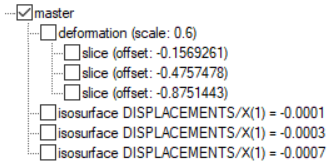
\includegraphics[width=0.5\textwidth]{figures/chapter-data-management/layers-tree-diagram}
    \decoRule
    \caption{Diagram of a layer tree.}
    \label{fig:layers-tree}
\end{figure}

The visualization of the master layer is in Figure \ref{fig:beam-master-layer}.

\begin{figure}[H]
    \centering
    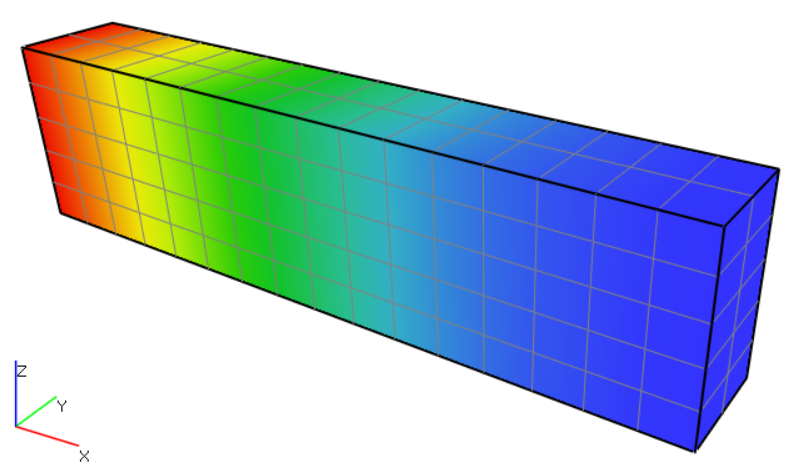
\includegraphics[width=0.7\textwidth]{figures/chapter-data-management/beam-master-layer}
    \decoRule
    \caption[Visualization of a master layer]{Visualization of a master layer with displacements in in Z axis.}
    \label{fig:beam-master-layer}
\end{figure}

The prototype implementation contains the following types of filters:

% layers, filters, vyjmenovat typy filtru, vytvoreni Surface vrstvy pro webovy postprocessor
% ke kazdemu typu filtru pridat obrazek z postprocessoru at je to zajimavy

\begin{itemize}

    \item \textbf{Deformation} -- Deformation filter performs the translation of the nodes of the parent mesh by the values of a vector field, usually the displacements field. The product is a layer that contains a deformed mesh as the one shown in Figure \ref{fig:beam-deformation-layer}.

    \begin{figure}[H]
        \centering
        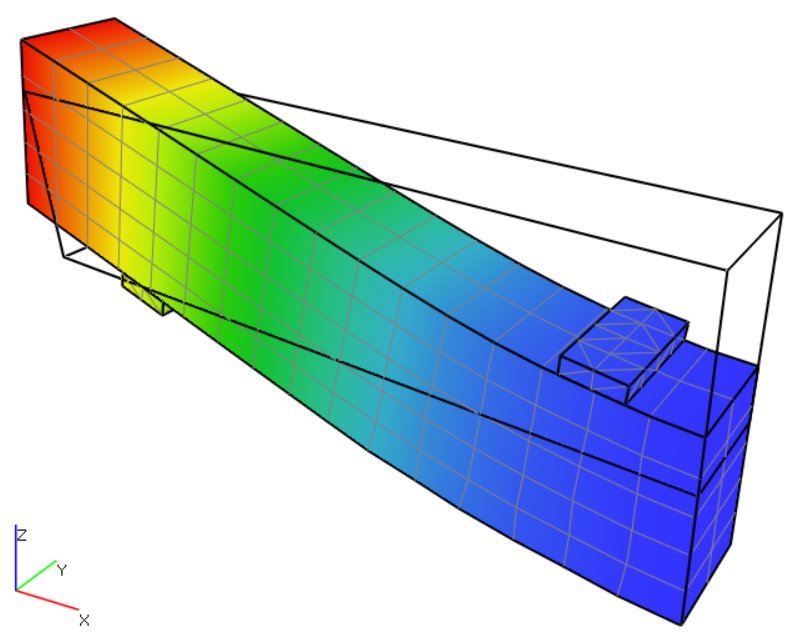
\includegraphics[width=0.7\textwidth]{figures/chapter-data-management/beam-deformation-layer}
        \decoRule
        \caption[Visualization of a deformation layer]{Visualization of a deformation layer with displacements in in Z axis.}
        \label{fig:beam-deformation-layer}
    \end{figure}
    
    As there is one-to-one mapping of the data values between the data locations in the parent mesh and the deformed mesh, there is no need for any transformation of the data or attributes. Also, to avoid the unnecessary copy of the data, the storage format supports a mechanism to share the data between a parent layer and its child layers. For this purpose, optional properties \code{DataFallbackLayerId}, \code{AttributeFallbackLayerId}, and \code{MeshFallbackLayerId} are available in Summary document. A post-processor checks the value of the fall-back properties before each request for a result, an attribute, or a mesh document to determine the layer id that should be used for the lookup.
    
    The geometry of a deformation layer is created once the deformation filter is applied on the parent layer. Therefore, the scale of the deformation has to be carefully selected as it cannot be modified after-the-fact during the post-processing. This is considered as a disadvantage of the chosen approach. The system helps to mitigate this problem by calculating a reasonable default value for the deformation scale (it is set to 10\%, relatively to the dimensions of the original mesh).

    \item \textbf{Slice} -- Slice filter generates a two-dimensional cross section through a three-dimensional mesh. A cross section is defined by a plane using a normal vector and an offset. Offset is a distance between the plane and the origin of the coordinate system. Example of a solution with multiple slice layers is depicted in Figure \ref{fig:beam-slice-layers}.
    
    \begin{figure}[H]
        \centering
        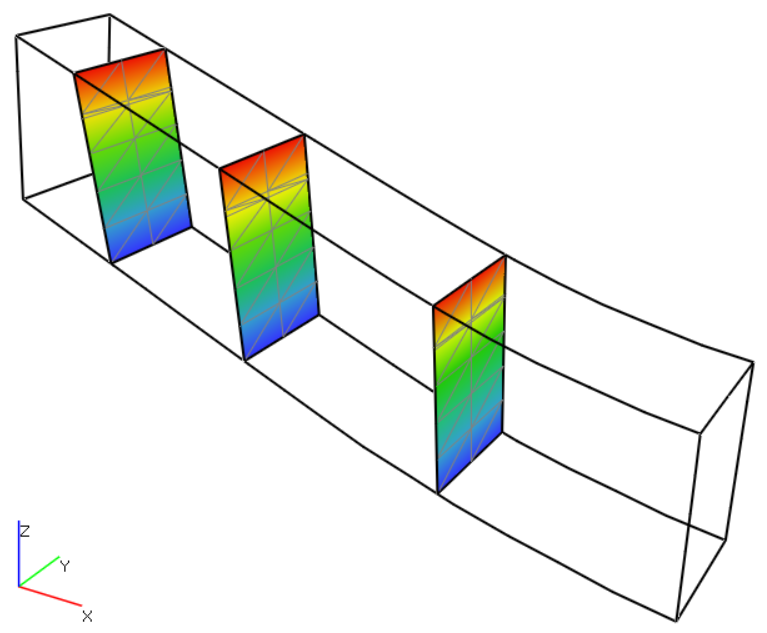
\includegraphics[width=0.7\textwidth]{figures/chapter-data-management/beam-slice-layers}
        \decoRule
        \caption[Visualization of multiple slice layers]{Visualization of multiple slice layers with displacements in X axis.}
        \label{fig:beam-slice-layers}
    \end{figure}

    Natural improvement of the slice filter could be the ability to automatically generate a sequence of parallel slices with an uniform distance between them. This will be a subject of a future work.
    
    \item \textbf{Iso-surface} -- Iso-surfaces are two-dimensional surfaces following a constant value of a data component. They help to visualize the gradient of a field inside the volume of a domain. Examples of three iso-surface filters are shown in Figure \ref{fig:beam-isosurface-layers}.
    
    \begin{figure}[H]
        \centering
        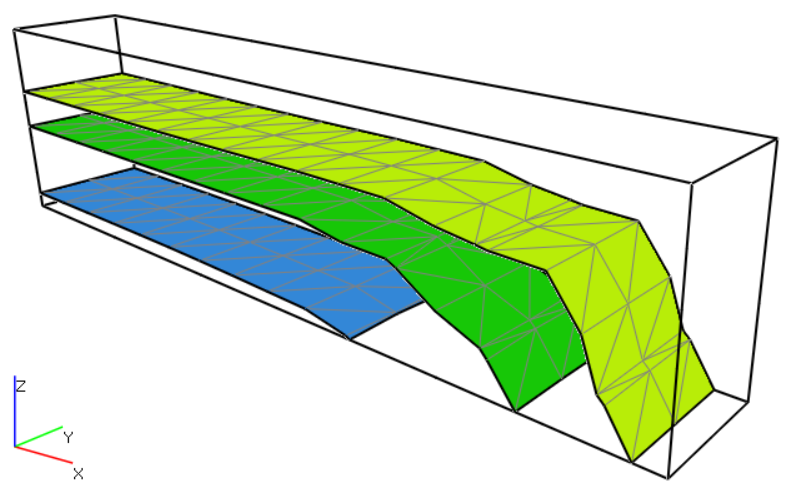
\includegraphics[width=0.7\textwidth]{figures/chapter-data-management/beam-isosurface-layers}
        \decoRule
        \caption[Visualization of multiple iso-surface layers]{Visualization of multiple iso-surface layers with displacements in X axis.}
        \label{fig:beam-isosurface-layers}
    \end{figure}

    \item \textbf{Attribute selection} -- Attribute selection filter allows to choose mesh entities (usually elements) having a particular attribute assigned (e.g., material property) and propagate them into a new layer, filtering out the other entities, that does not have the attribute assigned. In Figure \ref{fig:beam-attribute-selection-layer} there is shown how the attribute selection filter can be used to create a layer that contains only the one-dimensional elements of the original mesh.
    
    \begin{figure}[H]
        \centering
        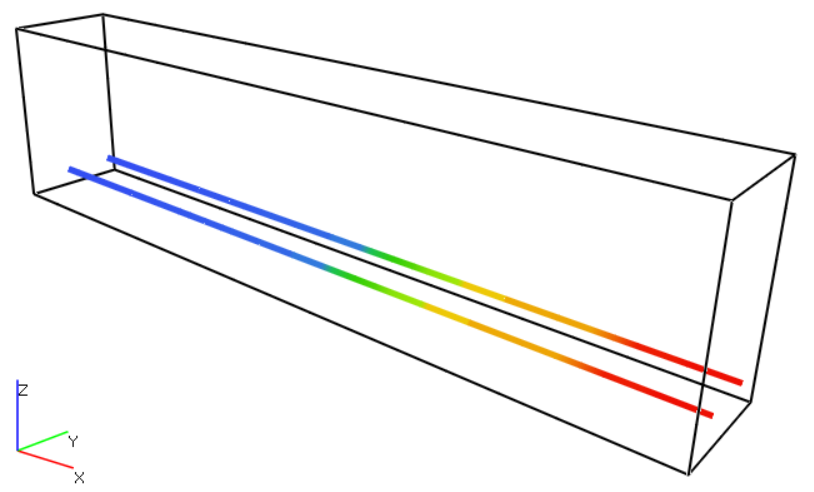
\includegraphics[width=0.7\textwidth]{figures/chapter-data-management/beam-attribute-selection-layer}
        \decoRule
        \caption{Visualization of an attribute selection layer.}
        \label{fig:beam-attribute-selection-layer}
    \end{figure}

    \item \textbf{Surface} -- Surface filter is a helper transform that produces a surface representation of a given mesh and maps the corresponding data and attributes onto the surface. It allows to significantly simplify the implementation of a post-processor. The prototype implementation of the web-based post-processor is able to visualize only a mesh that consists of simple triangles. To be able to visualize all types of elements (as shown in Figure \ref{fig:supported-cell-types}) the post-processor requests a creation of a surface layer for each layer containing 3D elements. The hard work is offloaded to the server and the implementation of the post-processor is kept as simple as possible with low memory and CPU requirements. Figure \ref{fig:beam-surface-layer} shows the visualization of a surface layer. Notice the triangles instead of quads on the surface. To preserve the identity of the original finite elements, the ids of elements can be tracked using a dedicated attribute document.

    \begin{figure}[H]
        \centering
        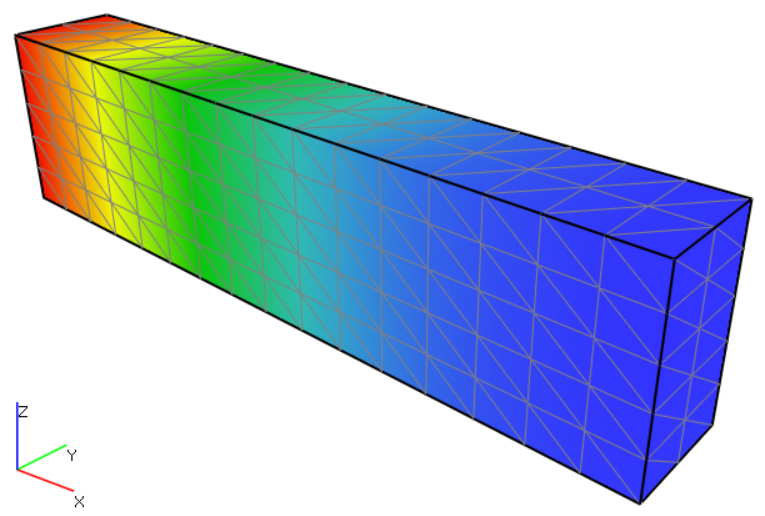
\includegraphics[width=0.7\textwidth]{figures/chapter-data-management/beam-surface-layer}
        \decoRule
        \caption{Visualization of a surface layer.}
        \label{fig:beam-surface-layer}
    \end{figure}

\end{itemize}

There are also ideas for other filters that are not yet implemented, e.g., Clip filter that creates a section through a mesh, but preserves (unlike Slice filter) the geometry behind the cut, or Stream-lines filter that enables to visualize a flow field by creating the tangent lines to the velocity vectors of the field.

As stated, a post-processor does not need to implement the visual filters itself. Filters are the integral part of the storage format and there is an dedicated service component that does all the manipulations with the format. A post-processor provides just a user interface for the filter definition and for the layer tree management. Typically, it has a tree view that displays the current layer tree, similar to the one in Figure \ref{fig:layers-tree}, where the user can turn on or off a particular layer or change the display mode of the current layer. When a filter layer is selected, a post-processor also displays the outline of its parent layer to be able to see the relationship of both layers. E.g. a deformation layer can be compared to the undeformed geometry, or the position of a slice layer can be put into context of its parent mesh.

The post-processing involves a number of features that are not handled externally as they cannot be represented persistently by the storage format. An example of such feature is the visualization of vector fields using arrows as shown in Figure \ref{fig:beam-vectors}. It is not a good candidate for a layer filter as vector arrows does not have static geometry. A user may want to change a scale of the arrows or move the origin of the arrows. A downside is the requirement to load all the components of a vector field into the memory at once to be able to build a visual representation. Therefore, this feature is only implemented in the feature-rich desktop post-processor for the time being.

\begin{figure}[H]
    \centering
    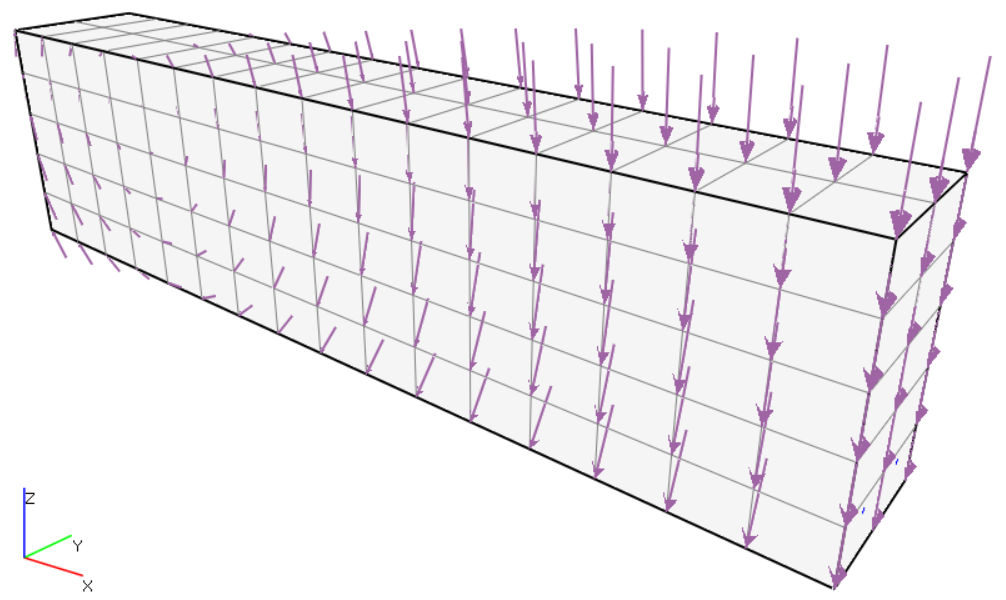
\includegraphics[width=0.7\textwidth]{figures/chapter-data-management/beam-vectors}
    \decoRule
    \caption{Example of the vector field visualization.}
    \label{fig:beam-vectors}
\end{figure}

One of the key features of a post-processor is the ability to map a data value, which is a floating-point number, to a color in color scale that is used to render a mesh surface. The mapping of the color can be configured. The implementation contains several predefined types of color scales including gray-scale, separated-by-zero\footnote{\todo{TODO: explain SeparatedByZero color scale}}, or a user-defined color scale type. There are two modes for calculating a color between the data locations -- standard interpolation and quantization, i.e., dividing the whole color scale into a few buckets, each corresponding to a different range of data values, and applying a constant color for each value in the range. In the implemented post-processor, this technique is called the iso-areas color scale and an example is shown in Figure \ref{fig:beam-isoareas-shader}. The iso-areas feature cannot be represented using the storage format. To avoid an ad-hoc generation of the corresponding geometry, which would be difficult to implement and would significantly degrade the performance, iso-areas feature is implemented purely inside the OpenGL pipeline using the special pixel shader\footnote{\todo{TODO: explain pixel shader}}.

% TODO: rozvinout vysvetleni barevne skaly: pridat diskretni barevnou skalu, pridat obrazek s element property?

\begin{figure}[H]
    \centering
    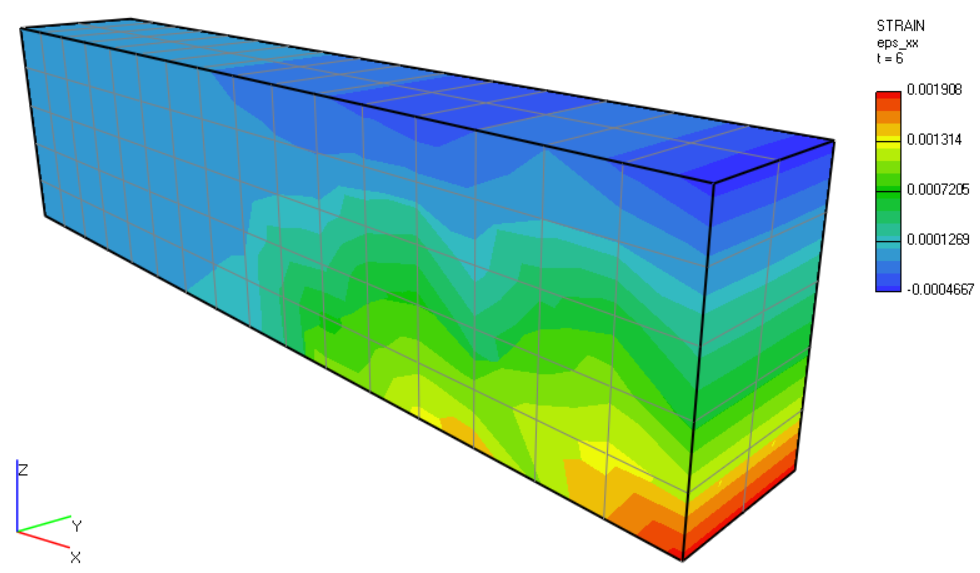
\includegraphics[width=0.75\textwidth]{figures/chapter-data-management/beam-isoareas-shader}
    \decoRule
    \caption{Iso-areas visualization of the xx component of the stress tensor.}
    \label{fig:beam-isoareas-shader}
\end{figure}


\section{Implementation details}
\label{sec:implementation-details}

The components of the data management system and their relations were outlined in Figure \ref{fig:FEA-architecture} and Figure \ref{fig:FEA-workflow}. This section discusses the implementation details of the application components based on the system design set out in the previous sections. The implementation of each component is discussed, including the programming languages, technologies, external providers, or libraries used in the prototype implementation of the application.

The architecture of the data management system is designed as modular and it consists of several isolated services. The full list of services needed either for remote or local post-processing follows. If there is no need or desire to run the system in the distributed environment, one can simply use only the components necessary to post-process the simulation results locally. These are two components -- the FEM results converter and the desktop post-processor.

It is worth noting that the prototype implementation uses the Microsoft Azure public cloud as an enviroment to test and demonstrate the whole system. However, any other cloud provider can be used in production. The system can also be run on-premises if there is any concern about data privacy.

\subsection*{Project data storage}

Project-related data are stored in the SQL database. The ER model depicted in Figure \ref{fig:FEA-db-schema-results} is mapped on the database schema consisting of tables Projects, Simulations, Solutions, and Layers. There is also the table Users that holds the information about the owners and collaborators connected with a particular project.

Microsoft SQL Server is used as the underlying relational database management system, specifically, its cloud-based version that runs as a platform-as-a-service in Microsoft Azure cloud.

\subsection*{FEM results storage}

FEM results converted to the proposed format are represented by a series of JSON documents. In case of the remote storage, documents are stored in a blob storage. The Microsoft Azure storage account is used as a provider for the blob storage service. The name of each document follows predefined convention so it can be easily constructed from the document index retrieved from the solution object stored in the relational database. The name of each blob follows the pattern:

\file{\{Layer-id-GUID\}/\{document-index\}.\{document-type\}.json}
%\footnote{The example of a document URI:\par \file{https://storage-account-name.blob.core.windows.net/fea-layers/3626f2ca-79d6-427b-a98f-19f86144c4ae/1.result.json}}

\noindent
In case of the local storage, the documents are stored in the local file system. The documents corresponding to a single layer are stored in a single folder and the paths and the names of the files are in the following form:

\file{\{path-to-folder\}/\{Layer-id-GUID\}/\{document-index\}.\{document-type\}.json}
%\footnote{The example of the path to a document in the local file system:\par \file{C:/Solutions/3fe47370-fb09-4c17-9bb7-0e75807d531f/4.result.json}}

\subsection*{FEM results converter}

FEM results converter is the core component of the data management system. It does implement all the necessary operations that query or manipulate the data in the proposed layer-based storage format. It is designed as an independent service that can run either in a remote or a local environment. It supports three deployment options:

\begin{enumerate}
    \item It works as a stand-alone console application that exposes command-line interface.
    \item It can run as a background task on the remote server, communicating via http requests.
    \item It can be directly referenced as a third party library by the post-processor, which eliminates the overhead of the communication interface.
\end{enumerate}

The FEM results converter component supports the following commands. (The commands can either be called directly by the post-processor, triggered by the message sent over the network, or even entered manually to the terminal as command-line arguments.)

\begin{itemize}
    \item \keyword{import} -- converts the output from a FEM solver to the universal storage format. (GiD and VTK file formats are currently supported.) The command creates a new solution with a single layer in it -- the master layer.
    \item \keyword{filter} -- creates a new layer by applying the requested filter on the specified parent layer.
    \item \keyword{list} -- enumerates all the layers in the solution. It is used to present the current layer tree to the user.
    \item \keyword{delete} -- deletes a layer.
    \item \keyword{help} -- displays more information on a specific command.
\end{itemize}

The filter command at first downloads the solution object from its storage location, then it retrieves the documents corresponding to a specific layer from either the remote blob storage, or the local file system, then it applies the requested filter on the layer's documents and generates the new filter layer consisting of transformed data. Finally, the layer tree is then updated to contain this new layer. As soon as any new layer is generated, it is considered as immutable and cannot be modified by any command. This simple principle prevents the conflicts when accessing the layer documents simultaneously from multiple locations, eliminates the consistency issues, and helps to avoid any need for sychronization mechanisms.

Both the import and the filter commands support the compression of the layer data. There is an optional argument for specifying the name of compression method and additional list of parameters that varies by the chosen compression method. E.g., the SVD compression method, accepts either ``error'' or ``size'' parameter (see Chapter \ref{chapter:SVD} for details). To support the SVD compression the converter component references the \textit{RedSVD} \cite{XXX} library that provides the compression method with the optimized algorithms for matrix decompositions.

The FEM results converter is implemented in C\# language and targets .NET Core framework, which among other things ensures cross-platform availability. The component can be either hosted as a webjob inside the Azure App Service (on a dedicated virtual server), or run on demand as a serverless\footnote{\todo{TODO: explain serverless}} application using the Azure Functions infrastructure.

\subsection*{Web API service}
% Storage format nemuze existovat sam o sobe. Jeho soucasti je cloud-based API, ktere s nim umoznuje manipulovat, vytvaret vrstvy, odpovidat na dotazy...
% ASP.NET Core
% Aggregation, Communication API providing, REST API, interface, backend providing project info
% Entity framework pro OR mapovani relacni databaze

\todo{TODO: \ldots}

\subsection*{Web post-processor}
% Presentation layer, Frontend, Data consuming and presenting
% zobrazuje data pouze z remote storage
% zevrubne popsat implementaci weboveho post-procesoru - z jakych soucasti se sklada, jak komunikuje se serverem
% Dekomprese: prenasobeni matic - staci jeden radek. ... 
% Webový browser, WebGL, THREE.js, Aurelia, Typescript, Command line tool (shell), veškeré zpracování příkazů na serveru, na klient se budou posílat jen grafické buffery
% Jak probiha komunikace s API a dotaz na vrstvy. Jak probiha cely proces dotazu a zobrazeni dat ve webovem postprocesoru. Jak funguje RemoteSolutionController. Remote/Local solutions - neni rozdil, postprocessor je tenky klient

\todo{TODO: \ldots}

\subsection*{Desktop post-processor}
% zobrazuje data z local i z remote storage
% odkazat se na kapitoly 4,5 - plynule navazat na dalsi kapitolu (Mesh visualization)

\todo{TODO: \ldots}
